\documentclass{article}

\usepackage{caption}

\usepackage{multirow}

\usepackage{graphicx}
\setlength{\abovecaptionskip}{10pt plus 3pt minus 2pt}
\setlength{\belowcaptionskip}{10pt plus 3pt minus 2pt}

\usepackage[margin=1in]{geometry}

\usepackage{hyperref}
\hypersetup{
    pdfborderstyle={/S/U/W 1},
    colorlinks=true,
    linkcolor=blue,
    filecolor=magenta,
    urlcolor=cyan,
}

\usepackage{algorithm,algpseudocode}

\usepackage{xcolor}
\usepackage{listings}
\lstdefinestyle{DOS}{
    backgroundcolor=\color{lightgray},
    basicstyle=\scriptsize\color{black}\ttfamily
}

\title{
CSE 5441 (Fall 2019, Dr. Jones)\\
\large \texttt{OpenMP} (Lab 3)
}
\author{
Caleb Lehman \\
\href{mailto:lehman.346@osu.edu}{lehman.346@osu.edu}
}

\begin{document}
\maketitle

\section*{Overview}
\label{sec:overview}

For this lab, I made slight modifications to my serial \texttt{C} program to
perform Adaptive Mesh Refinement (AMR)\footnote{See lab 1 or project
descriptions for details about AMR computation.} to work in parallel using the
Intel implementation of the OpenMP API.  I created 2 programs,
\texttt{disposable} and \texttt{persistent}, which mirror the disposable and
persistent thread models used in the previous lab. In particular, the
\texttt{disposable} code opens a new parallel region for each iteration, while
the \texttt{persistent} code has a single parallel region encompassing the
entire convergence loop, inside of which, each iteration is divided between the
threads.

\section*{Tests}
\label{sec:tests}

\subsection*{Environment}
\label{subsec:environment}

The program was developed and tested on the
\href{https://www.osc.edu/resources/technical_support/supercomputers/pitzer}{Pitzer
cluster} at the \href{https://www.osc.edu/}{Ohio Supercomputer Center}.

For development, I loaded the \texttt{intel/18.0.3} module, which allowed the
program to be compiled with version 18.0.3 of the \texttt{icc} C-compiler.

For testing, I loaded the \texttt{python/3.6-conda5.2} module, which loads a
python environment with the \texttt{NumPy}, \texttt{SciPy}, and
\texttt{Matplotlib} packages, amoung others. \texttt{Python} is only necessary
for collecting and plotting the data from testing, not for the actual exectuion
of the program.

\subsection*{Timing}
\label{subsec:timing}

I collected timing data using the same 4 methods as the first lab:
\texttt{time}, \texttt{clock}, and \texttt{clock\textunderscore gettime} from
the \texttt{"time.h"} header; and the \texttt{UNIX} utility \texttt{time}.

As with the second lab, I didn't use the results from the \texttt{clock} function from the
\texttt{"time.h"} header, since it reports CPU time, not wall time. The other
methods all returned values within 1 second of each other. The \texttt{time}
function declared in \texttt{"time.h"} returns an integer number of seconds,
but the other two methods return with sub-second precision.  \emph{For
consistency, I used the \texttt{clock\textunderscore gettime} function for all
results in this report}.

\subsection*{Test Files}
\label{subsec:test_files}

Dr. Jones provided the \texttt{testgrid\textunderscore 400\textunderscore
12206} test file.  As part of lab 1, I reduced the $\alpha$ (affect rate) and
$\varepsilon$ parameters until the serial runtime increased into the 3 to 6
minute range. In particular, I selected $\alpha = 0.01$ and $\varepsilon =
0.02$, for which the serial program completed in 261 seconds.

The above approach of changing the $\alpha$ and $\epsilon$ parameters allows us
to make the programs run longer, but doesn't affect the actual length of each
iteration. With only 12206 boxes, each iteration is fairly short (on the order
of $\frac{261\textrm{ sec}}{1589637} = 0.16\textrm{ms}$ per iteration), so it is
expected the overhead of synchronizing threads would inhibit parallelizing
beyond a small number of threads. In order to investigate this, I generated
another test file, \texttt{testgrid\textunderscore 1000\textunderscore 296793},
which has more boxes and therefore longer iterations.

\begin{table}[h]
    \centering
    \begin{tabular}{|c|c|c|c|c|c|}
        \hline
        test & \texttt{\#} rows & \texttt{\#} cols & \texttt{\#} boxes & mean \texttt{\#} neighbors & std. dev. \texttt{\#} neighbors \\
        \hline
        \hline
        \texttt{testgrid\textunderscore 400\textunderscore 12206} & 400 & 400 & 12206 & 5.89 & 1.55 \\
        \texttt{testgrid\textunderscore 1000\textunderscore 296793} & 1000 & 1000 & 296793 & 4.79 & 1.57 \\
        \hline
    \end{tabular}
    
    \caption{Basic statistics for my test files. Note that the file in the
    second row was engineered to have many boxes.}

\end{table}

\newpage
\section*{Results}
\label{sec:results}

The output for each test case was consistent across all variations and was as follows:
\begin{itemize}
    \item \texttt{testgrid\textunderscore 400\textunderscore 12206}: 1589637 iterations, $(max, min) = (0.085900, 0.084182)$
    \item \texttt{testgrid\textunderscore 1000\textunderscore 296793}: 51684 iterations, $(max, min) = (0.000000, 0.000000)$
\end{itemize}

The relevant runtimes for the serial, \texttt{pthreads}, and \texttt{OpenMP}
versions on each of the two test cases are plotted in the figure below. Note
that the \texttt{OpenMP} \texttt{persistent} and \texttt{disposable} versions
perform nearly identically. This suggests that (at least this \texttt{Intel}
implementation of) \texttt{OpenMP} uses some sort of thread pool that creates
the threads early in the program and doesn't destroy them until the end, simply
assigning threads at the beginning of each parallel section.

For the smaller test case, \texttt{OpenMP} outperformed \texttt{pthreads}, both
yielding consistently lower runtimes, as well as scaling better (improved performance
up to 12 threads). I suspect this has to do with how optimized the threading
mechanisms are for their various tasks. In particular, in the \texttt{pthreads}
implementation, I had to manually write to code to create and destroy threads,
as well as create, pass, and collect the structures/paramaters passed to the
threads. While this certainly provides more flexibility that then basic
\texttt{OpenMP} \texttt{pragma} directives, which are limited by comparison,
the corresponding operations in the \texttt{OpenMP} implementation are almost
certainly highly optimized. In this smaller test case, each iteration is
relatively short, so the overhead from basic thread management most likely is
significant for the overall runtime.

For the larger test case on the other hand, each iteration is longer, so the
basic thread management overhead is less impactful compared to actual
parallelization of the work.  In this case, \texttt{OpenMP} was outperformed by
the \texttt{persistent} version of the \texttt{pthreads} program. One
explanation for this is that my use of \texttt{pthreads} was specifically
targetted at this particular problem, while the \texttt{OpenMP} directives are
more general (by design) and therefore may not be as well-suited for this
specific computation.

\vspace{1em}
\begin{minipage}{\linewidth}
    \centering
    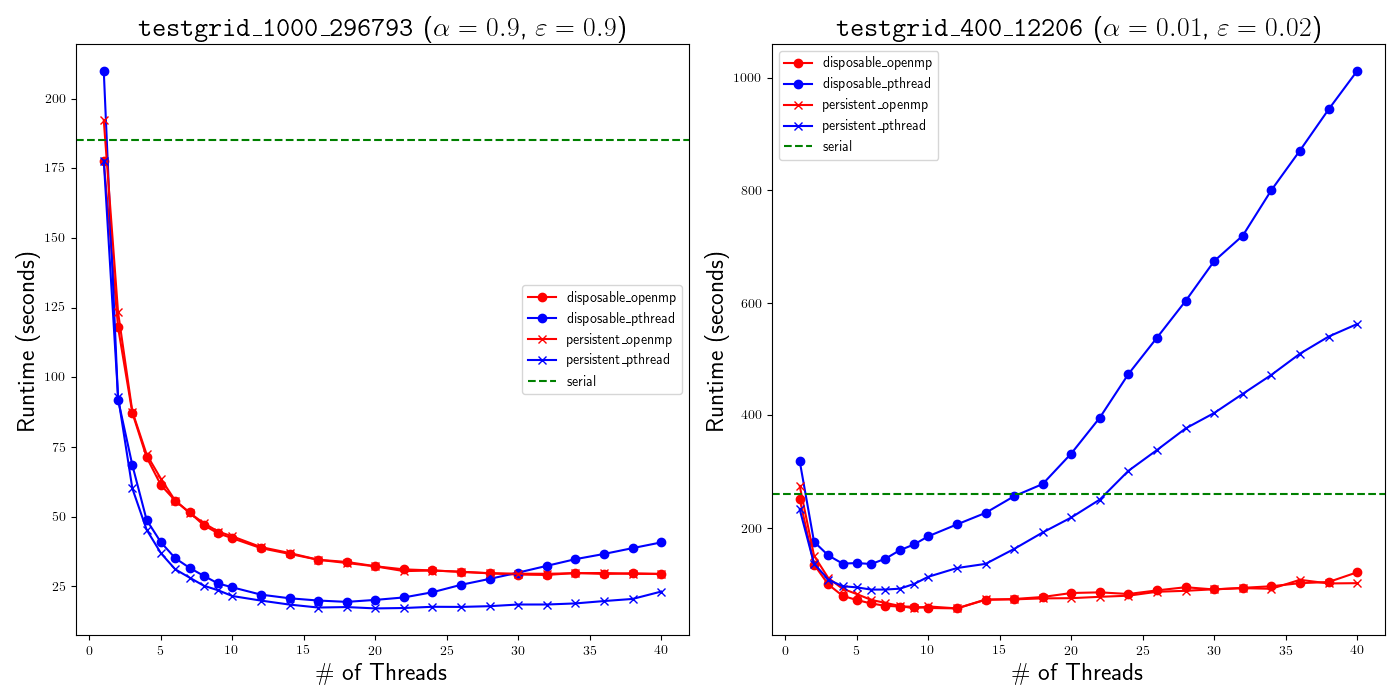
\includegraphics[width=.8\linewidth]{../results/plot.png}

    \captionof{figure}{The runtimes of the parallel versions (\texttt{pthreads}
    and \texttt{OpenMP}) of the program plotted against the number of threads
    used. Serial runtime is included for comparison. Note that \texttt{OpenMP}
    \texttt{persistent} and \texttt{disposable} versions consistently perform
    nearly identically.}

    \label{fig:runtimes}
\end{minipage}

It is worth noting that the \texttt{OpenMP} parallelization was much less
intrusive compared to the \texttt{pthreads} parallelization. The
\texttt{persistent} version required a few \texttt{pragma} directives and some
code to compute the workload division for each thread, but used much less new
code than the corresponding \texttt{pthreads} version.  The \texttt{disposable}
version required just 2-3 \texttt{pragma}s to parallelize and achieved just as
good results as the \texttt{persistent} version. Furthermore, both versions
compile\footnote{not including harmless warnings about unrecognized
\texttt{pragma}s} and execute correctly as serial programs when compiled without
\texttt{OpenMP}.

Finally, since the \texttt{OpenMP} specifications don't have many strict
requirements about using the exact number of threads requested in each
parallel region, I included checks in both of the programs to verify that the
number of threads was the same as the number requested. For all reasonable
requests (between 1 and 40 threads on \texttt{Pitzer}), I never got an
unexpected number of threads.

\section*{Project Usage}
\label{sec:project}

This section details basic commands needed to build and run the project and is
only applicable for the code submission corresponding to this report. For full
details, see the \texttt{README} included in the code submission.

\subsection*{Building}
\label{subsec:building}

To build the \texttt{disposable} and \texttt{persistent} executables, navigate
to the top level of the submitted directory and build as follows:

\begin{lstlisting}[style=DOS]
# Ensure that you have icc compiler

$ make
$ ls
... persistent disposable ...
\end{lstlisting}

\subsection*{Running}
\label{subsec:running}

The syntax to run the program is:

\begin{lstlisting}[style=DOS]
$ ./[program] [affect-rate] [epsilon] [num-threads] <[test-file]
\end{lstlisting}
where \texttt{program} is one of \texttt{persistent}, \texttt{disposable}
and \texttt{num-threads} is positive integer number of threads.

\end{document}
